%\documentclass[12pt,twoside]{article}
\documentclass{article}
\usepackage[a4paper,margin=1in]{geometry}

\usepackage[dvipsnames]{xcolor}
\usepackage{tikz,graphicx,amsmath,amsfonts,amscd,amssymb,mathrsfs, bm,cite,epsfig,epsf,url}
\usepackage[hang,flushmargin]{footmisc}
\usepackage[colorlinks=true,urlcolor=blue,citecolor=blue]{hyperref}
\usepackage{amsthm,multirow,wasysym,appendix}
\usepackage{array,subcaption} 
% \usepackage[small,bf]{caption}
\usepackage{bbm}
\usepackage{pgfplots}
\usetikzlibrary{spy}
\usepgfplotslibrary{external}
\usepgfplotslibrary{fillbetween}
\usetikzlibrary{arrows,automata}
\usepackage{thmtools}
\usepackage{blkarray} 
\usepackage{textcomp}
\usepackage{float}
%\usepackage[left=0.8in,right=1.0in,top=1.0in,bottom=1.0in]{geometry}


\usepackage{times}
\usepackage{amsfonts}
\usepackage{amsmath}
\usepackage{latexsym}
\usepackage{color}
\usepackage{graphics}
\usepackage{enumerate}
\usepackage{amstext}
\usepackage{blkarray}
\usepackage{url}
\usepackage{epsfig}
\usepackage{bm}
\usepackage{hyperref}
\hypersetup{
    colorlinks=true,
    linkcolor=blue,
    filecolor=magenta,      
    urlcolor=blue,
}
\usepackage{textcomp}
%\usepackage[left=0.8in,right=1.0in,top=1.0in,bottom=1.0in]{geometry}
\usepackage{mathtools}
%\usepackage{minted}
\usepackage{gensymb}

\usepackage{graphicx}
\usepackage{float}
\usepackage[justification=centering,singlelinecheck=true]{caption}
\usepackage{subcaption}   
\usepackage{caption}
\captionsetup[figure]{skip=5pt}   % ← distance between figure and caption

%% Probability operators and functions
%
% \def \P{\mathrm{P}}
\def \P{\mathrm{P}}
\def \E{\mathrm{E}}
\def \Var{\mathrm{Var}}
\let\var\Var
\def \Cov {\mathrm{Cov}} \let\cov\Cov
\def \MSE {\mathrm{MSE}} \let\mse\MSE
\def \sgn {\mathrm{sgn}}
\def \R {\mathbb{R}}
\def \C {\mathbb{C}}
\def \N {\mathbb{N}}
\def \Z {\mathbb{Z}}
\def \cV {\mathcal{V}}
\def \cS {\mathcal{S}}

\newcommand{\RR}{\ensuremath{\mathbb{R}}}

\DeclareMathOperator*{\argmin}{arg\,min}
\DeclareMathOperator*{\argmax}{arg\,max}
\newcommand{\red}[1]{\textcolor{red}{#1}}
\newcommand{\blue}[1]{\textcolor{blue}{#1}}
\newcommand{\green}[1]{\textcolor{ForestGreen}{ #1}}
\newcommand{\fuchsia}[1]{\textcolor{RoyalPurple}{ #1}}



%
%% Probability distributions
%
%\def \Bern    {\mathrm{Bern}}
%\def \Binom   {\mathrm{Binom}}
%\def \Exp     {\mathrm{Exp}}
%\def \Geom    {\mathrm{Geom}}
% \def \Norm    {\mathcal{N}}
%\def \Poisson {\mathrm{Poisson}}
%\def \Unif    {\mathrm {U}}
%
\DeclareMathOperator{\Norm}{\mathcal{N}}

\newcommand{\bdb}[1]{\textcolor{red}{#1}}

\newcommand{\ml}[1]{\mathcal{ #1 } }
\newcommand{\wh}[1]{\widehat{ #1 } }
\newcommand{\wt}[1]{\widetilde{ #1 } }
\newcommand{\conj}[1]{\overline{ #1 } }
\newcommand{\rnd}[1]{\tilde{ #1 } }
\newcommand{\rv}[1]{ \rnd{ #1}  }
\newcommand{\rx}{\rnd{ x}  }
\newcommand{\ry}{\rnd{ y}  }
\newcommand{\rz}{\rnd{ z}  }
\newcommand{\ra}{\rnd{ a}  }
\newcommand{\rb}{\rnd{ b}  }
\newcommand{\rpc}{\widetilde{ pc}  }
\newcommand{\rndvec}[1]{\vec{\rnd{#1}}}

\def \cnd {\, | \,}
\def \Id { I }
\def \J {\mathbf{1}\mathbf{1}^T}

\newcommand{\op}[1]{\operatorname{#1}}
\newcommand{\setdef}[2]{ := \keys{ #1 \; | \; #2 } }
%\newcommand{\set}[2]{ \keys{ #1 \; | \; #2 } }
\newcommand{\sign}[1]{\op{sign}\left( #1 \right) }
\newcommand{\trace}[1]{\op{tr}\left( #1 \right) }
\newcommand{\tr}[1]{\op{tr}\left( #1 \right) }
\newcommand{\inv}[1]{\left( #1 \right)^{-1} }
%\newcommand{\abs}[1]{\left| #1 \right|}
\newcommand{\sabs}[1]{| #1 |}
\newcommand{\keys}[1]{\left\{ #1 \right\}}
\newcommand{\sqbr}[1]{\left[ #1 \right]}
\newcommand{\sbrac}[1]{ ( #1 ) }
\newcommand{\brac}[1]{\left( #1 \right) }
\newcommand{\bbrac}[1]{\big( #1 \big) }
\newcommand{\Bbrac}[1]{\Big( #1 \Big)}
\newcommand{\BBbrac}[1]{\BIG( #1 \Big)}
\newcommand{\MAT}[1]{\begin{bmatrix} #1 \end{bmatrix}}
\newcommand{\sMAT}[1]{\left(\begin{smallmatrix} #1 \end{smallmatrix}\right)}
\newcommand{\sMATn}[1]{\begin{smallmatrix} #1 \end{smallmatrix}}
\newcommand{\PROD}[2]{\left \langle #1, #2\right \rangle}
\newcommand{\PRODs}[2]{\langle #1, #2 \rangle}
\newcommand{\der}[2]{\frac{\text{d}#2}{\text{d}#1}}
\newcommand{\pder}[2]{\frac{\partial#2}{\partial#1}}
\newcommand{\derTwo}[2]{\frac{\text{d}^2#2}{\text{d}#1^2}}
\newcommand{\ceil}[1]{\lceil #1 \rceil}
\newcommand{\Imag}[1]{\op{Im}\brac{ #1 }}
\newcommand{\Real}[1]{\op{Re}\brac{ #1 }}
%\newcommand{\norm}[1]{\left|\left| #1 \right|\right| }
\newcommand{\norms}[1]{ \| #1 \|  }
\newcommand{\normProd}[1]{\left|\left| #1 \right|\right| _{\PROD{\cdot}{\cdot}} }
\newcommand{\normTwo}[1]{\left|\left| #1 \right|\right| _{2} }
\newcommand{\normTwos}[1]{ \| #1  \| _{2} }
\newcommand{\normZero}[1]{\left|\left| #1 \right|\right| _{0} }
\newcommand{\normTV}[1]{\left|\left| #1 \right|\right|  _{ \op{TV}  } }% _{\op{c} \ell_1} }
\newcommand{\normOne}[1]{\left|\left| #1 \right|\right| _{1} }
\newcommand{\normOnes}[1]{\| #1 \| _{1} }
\newcommand{\normOneTwo}[1]{\left|\left| #1 \right|\right| _{1,2} }
\newcommand{\normF}[1]{\left|\left| #1 \right|\right| _{\op{F}} }
\newcommand{\normLTwo}[1]{\left|\left| #1 \right|\right| _{\ml{L}_2} }
\newcommand{\normNuc}[1]{\left|\left| #1 \right|\right| _{\ast} }
\newcommand{\normOp}[1]{\left|\left| #1 \right|\right|  }
\newcommand{\normInf}[1]{\left|\left| #1 \right|\right| _{\infty}  }
\newcommand{\proj}[1]{\mathcal{P}_{#1} \, }
\newcommand{\diff}[1]{ \, \text{d}#1 }
\newcommand*\Diff[1]{\mathop{}\!\mathrm{d^#1}}
\newcommand{\vc}[1]{\boldsymbol{\vec{#1}}}
\newcommand{\rc}[1]{\boldsymbol{#1}}
\newcommand{\vx}{\vec{x}}
\newcommand{\vy}{\vec{y}}
\newcommand{\vz}{\vec{z}}
\newcommand{\vu}{\vec{u}}
\newcommand{\vv}{\vec{v}}
\newcommand{\vb}{\vec{\beta}}
\newcommand{\va}{\vec{\alpha}}
\newcommand{\vaa}{\vec{a}}
\newcommand{\vbb}{\vec{b}}
\newcommand{\vg}{\vec{g}}
\newcommand{\vw}{\vec{w}}
\newcommand{\vh}{\vec{h}}
\newcommand{\vbeta}{\vec{\beta}}
\newcommand{\valpha}{\vec{\alpha}}
\newcommand{\vgamma}{\vec{\gamma}}
\newcommand{\veta}{\vec{\eta}}
\newcommand{\vnu}{\vec{\nu}}
\newcommand{\rw}{\rnd{w}}
\newcommand{\rvnu}{\vc{\nu}}
\newcommand{\rvv}{\rndvec{v}}
\newcommand{\rvw}{\rndvec{w}}
\newcommand{\rvx}{\rndvec{x}}
\newcommand{\rvy}{\rndvec{y}}
\newcommand{\rvz}{\rndvec{z}}
\newcommand{\rvX}{\rndvec{X}}

% tell LaTeX to load ntheorem (with thmmarks) *before* thmtools
\usepackage[thmmarks]{ntheorem}  
\usepackage{thmtools}

\newtheorem{theorem}{Theorem}[section]
% \declaretheorem[style=plain,qed=$\square$]{theorem}
\newtheorem{corollary}[theorem]{Corollary}
\newtheorem{definition}[theorem]{Definition}
\newtheorem{lemma}[theorem]{Lemma}
\newtheorem{remark}[theorem]{Remark}
\newtheorem{algorithm}[theorem]{Algorithm}

% \theoremstyle{definition}
%\newtheorem{example}[proof]{Example}
%\declaretheorem[style=definition,qed=$\triangle$,sibling=definition]{example}
%\declaretheorem[style=definition,qed=$\bigcirc$,sibling=definition]{application}

%
%% Typographic tweaks and miscellaneous
%\newcommand{\sfrac}[2]{\mbox{\small$\displaystyle\frac{#1}{#2}$}}
%\newcommand{\suchthat}{\kern0.1em{:}\kern0.3em}
%\newcommand{\qqquad}{\kern3em}
%\newcommand{\cond}{\,|\,}
%\def\Matlab{\textsc{Matlab}}
%\newcommand{\displayskip}[1]{\abovedisplayskip #1\belowdisplayskip #1}
%\newcommand{\term}[1]{\emph{#1}}
%\renewcommand{\implies}{\;\Rightarrow\;}

% My macros

\def\Kset{\mathbb{K}}
\def\Nset{\mathbb{N}}
\def\Qset{\mathbb{Q}}
\def\Rset{\mathbb{R}}
\def\Sset{\mathbb{S}}
\def\Zset{\mathbb{Z}}
\def\squareforqed{\hbox{\rlap{$\sqcap$}$\sqcup$}}
\def\qed{\ifmmode\squareforqed\else{\unskip\nobreak\hfil
\penalty50\hskip1em\null\nobreak\hfil\squareforqed
\parfillskip=0pt\finalhyphendemerits=0\endgraf}\fi}

%\DeclareMathOperator*{\E}{\rm E}
%\DeclareMathOperator*{\argmax}{\rm argmax}
%\DeclareMathOperator*{\argmin}{\rm argmin}
%\DeclareMathOperator{\sgn}{sign}
\DeclareMathOperator{\supp}{supp}
\DeclareMathOperator{\last}{last}
%\DeclareMathOperator{\sign}{\sgn}
\DeclareMathOperator{\diag}{diag}
\providecommand{\abs}[1]{\lvert#1\rvert}
\providecommand{\norm}[1]{\lVert#1\rVert}
\def\vcdim{\textnormal{VCdim}}
\DeclareMathOperator*{\B}{\textbf{B}}

%\DeclarePairedDelimiter\ceil{\lceil}{\rceil}
%\DeclarePairedDelimiter\floor{\lfloor}{\rfloor}

\newcommand{\cX}{{\mathcal X}}
\newcommand{\cY}{{\mathcal Y}}
\newcommand{\cA}{{\mathcal A}}
\newcommand{\ignore}[1]{}
\newcommand{\ba}{\[\begin{aligned}}
\newcommand{\ea}{\end{aligned}\]}
\newcommand{\bi}{\begin{itemize}}
\newcommand{\ei}{\end{itemize}}
\newcommand{\be}{\begin{enumerate}}
\newcommand{\ee}{\end{enumerate}}
\newcommand{\bd}{\begin{description}}
\newcommand{\ed}{\end{description}}
\newcommand{\h}{\widehat}
\newcommand{\e}{\epsilon}
\newcommand{\mat}[1]{{\mathbf #1}}
%\newcommand{\R}{\mat{R}}
\newcommand{\0}{\mat{0}}
\newcommand{\M}{\mat{M}}

\newcommand{\D}{\mat{D}}
\renewcommand{\r}{\mat{r}}
\newcommand{\x}{\mat{x}}
\renewcommand{\u}{\mat{u}}
\renewcommand{\v}{\mat{v}}
\newcommand{\w}{\mat{w}}
\renewcommand{\H}{\text{0}}
\newcommand{\T}{\text{1}}
%\newcommand{\set}[1]{\{#1\}}
\newcommand{\xxi}{{\boldsymbol \xi}}
\newcommand{\ssigma}{{\boldsymbol \sigma}}
\newcommand{\Alpha}{{\boldsymbol \alpha}}
\newcommand{\tts}{\tt \small}
\newcommand{\hint}{\emph{hint}}
\newcommand{\matr}[1]{\bm{#1}}     % ISO complying version
\newcommand{\vect}[1]{\bm{#1}} % vectors

%\newcommand{\Var}{\mathrm{Var}}
%\newcommand{\Cov}{\mathrm{Cov}}

% New commands
\newcommand{\SP}{\mathbf{S}_{+}^n}
\newcommand{\Proj}{\mathcal{P}_{\mathcal{S}}}
%\DeclarePairedDelimiterX{\inp}[2]{\langle}{\rangle}{#1, #2}




\begin{document}

\noindent Professor Alex Spector\\
EN.585.743.81.SP25 Modeling Approaches to Cell and Tissue Engineering\\
Modeling Project\\
Johns Hopkins University\\
Student: Yves Greatti\\\

\section*{Introduction}
In Lecture 12, the polarization of the stem cell cytoskeleton as a function of
the stiffness of ECM is considered. A number of characteristics of cell/ECM
interaction, such as the modeling-predicted order parameter \cite{Zemel2010}
(Figure~\ref{fig:combined}(a)) or experiment-estimated myosin fiber intensity
\cite{Zemel2010} (Figure~\ref{fig:combined}(b)) demonstrate an
increase–saturation pattern as functions of ECM stiffness.
Use the 1-D model where the cell and ECM are presented by the active and
elastic springs, respectively \cite{Zemel2010}  (Figure~\ref{fig:1d-spring-model}) and show that the active force generated
by the cell, f$_a$, as a function of the ECM stiffness, has the same increase 
saturation pattern of behavior.


\begin{figure}[h!]
  \centering
  \begin{subfigure}[b]{0.45\textwidth}
    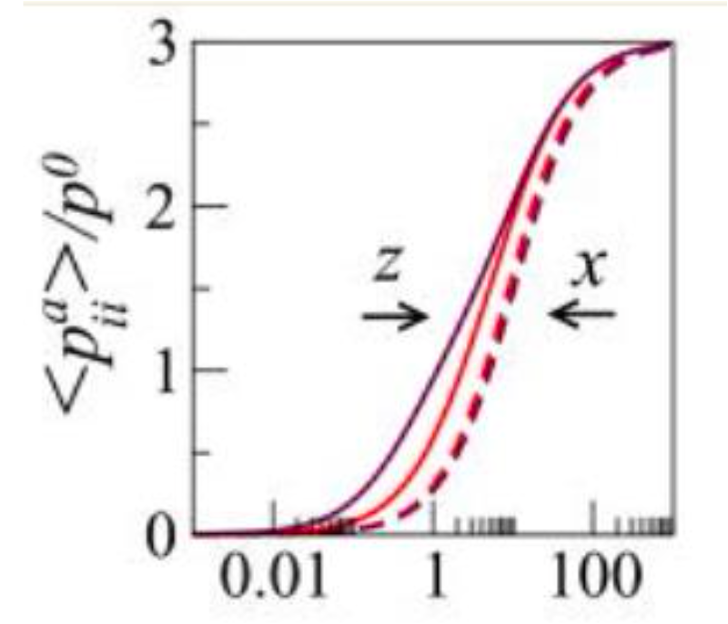
\includegraphics[width=\textwidth]{order_parameter}
    \caption{Normalized order parameter vs.\ \(\frac{E_m}{E_c}\).}
    \label{fig:order_parameter}
  \end{subfigure}
  \quad
  \begin{subfigure}[b]{0.45\textwidth}
    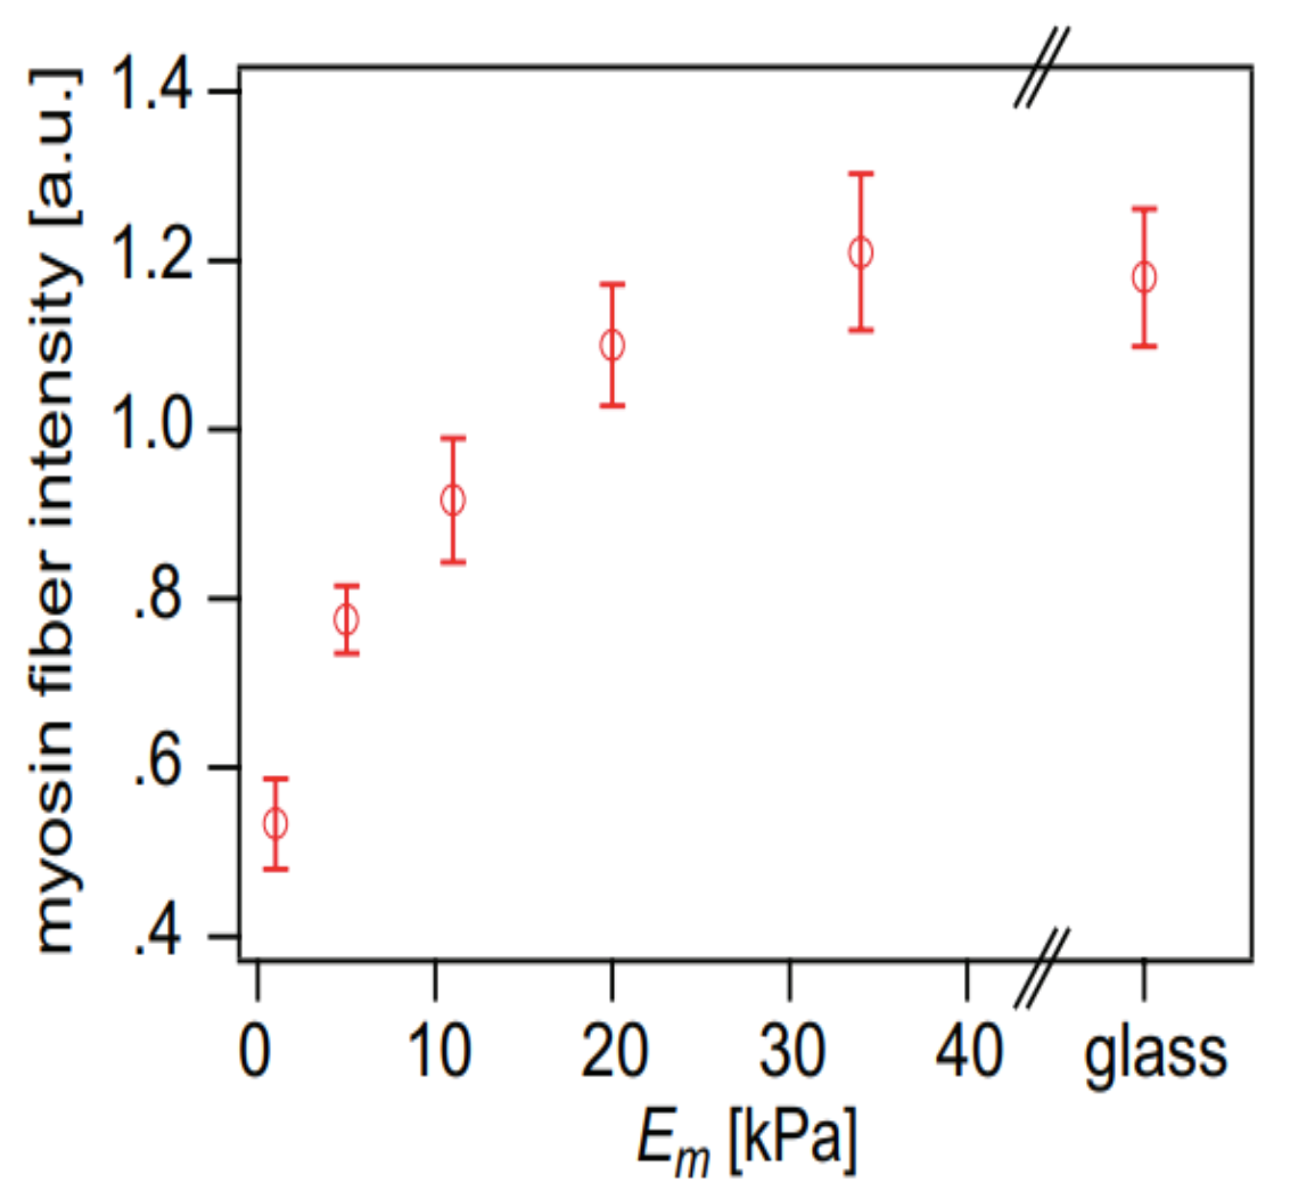
\includegraphics[width=\textwidth]{actomyosin}
    \caption{Myosin fibre intensity vs.\ \(E_m\).}
    \label{fig:myosin}
  \end{subfigure}
  \caption{(a) Order–parameter saturation. (b) Actomyosin‐intensity saturation.}
  \label{fig:combined}
\end{figure}

\section*{Derivation}

We want to show, using the 1D two‐spring model of cell and matrix (Figure~\ref{fig:1d-spring-model}),
that the cell’s active force \(f_a\) satisfies the equation:
\[
\frac{f^{a}}{f^{0}} = \alpha \,\frac{k_{m}}{\tilde{k}_{c} + k_{m}}
\]
At equilibrium:
\begin{align}
  k_c (l_c - l_c^R) &= k_m (l_m - l_m^R)  \label{eq:force-balance}\\
  l_c + l_m         &= l_c^0 + l_m^R      \label{eq:length-sum}
\end{align}

From \eqref{eq:length-sum}, 
\begin{equation}\label{eq:l_m}
  l_m = (l_c^0 + l_m^R) - l_c
\end{equation}

Substitute \eqref{eq:l_m} into the force-balance \eqref{eq:force-balance}:
\begin{align*}
  k_c (l_c - l_c^R)
  &= k_m \bigl(l_m - l_m^R\bigr) \nonumber\\
  &= k_m\bigl((l_c^0 + l_m^R) - l_c - l_m^R\bigr)\nonumber\\
  &= k_m (l_c^0 - l_c)\,. 
\end{align*}

Rearrange to solve for \(l_c\):
\begin{align*}
  k_c\,l_c - k_c\,l_c^R       &= k_m\,l_c^0 - k_m\,l_c \nonumber\\
  k_c\,l_c + k_m\,l_c         &= k_m\,l_c^0 + k_c\,l_c^R \nonumber\\
  (k_c + k_m)\,l_c            &= k_m\,l_c^0 + k_c\,l_c^R \nonumber\\
  l_c                         &= \frac{k_m\,l_c^0 + k_c\,l_c^R}{k_c + k_m}
\end{align*}

We have
\[
  l_c^R = l_c^0 + \Delta l_c^0,
\]
then
\begin{align*}
  l_c
  &= \frac{k_m\,l_c^0 + k_c\,(l_c^0 + \Delta l_c^0)}{k_c + k_m}\nonumber\\
  &= \frac{(k_m + k_c)\,l_c^0 + k_c\,\Delta l_c^0}{k_c + k_m}\nonumber\\
  &= l_c^0 + \frac{k_c}{k_c + k_m}\,\Delta l_c^0\,,
\end{align*}
so
\[
  \Delta l_c \;=\; l_c - l_c^0 \;=\; \frac{k_c}{k_c + k_m}\,\Delta l_c^0
\]

Introducing myosin polarization of the cytoskeleton fibers within the cell,  with 
\[
  \tilde{k}_c \;=\; (1 + \alpha)\,k_c \quad (\alpha>0)
\]
the cellular strain satisfies the equation
\[
  \frac{\Delta l_c}{l_c^0}
  = \frac{\tilde{k}_c}{\tilde{k}_c + k_m}\,\frac{\Delta l_c^0}{l_c^0}
\]

The active force is modeled as:
\[
  f^a = -\,\alpha\,k_c\,(l_c - l_c^R)
\]
from
\[
  \Delta l_c \;=\; l_c - l_c^0 \;=\; \,\frac{\tilde{k}_c}{\tilde{k}_c + k_m} \,\Delta l_c^0
\]

Thus:
\begin{align*}
l_c^R - l_c &= (l_c^R - l_c^0) + (l_c^0 - l_c) \\
&= \Delta l_c^0 - \frac{\tilde{k}_c}{\tilde{k}_c + k_m} \Delta l_c^0 \\
&= \left(1 - \frac{\tilde{k}_c}{\tilde{k}_c + k_m} \right) \Delta l_c^0 \\
&= \frac{k_m}{\tilde{k}_c + k_m} \Delta l_c^0
\end{align*}

Substituting back into the active force:
\[
f^a = -\alpha k_c (l_c - l_c^R) = \alpha k_c \left( \frac{k_m}{\tilde{k}_c + k_m} \Delta l_c^0 \right)
\]

Since the baseline force \(f^0\) is proportional to \(k_c \Delta l_c^0\):
\[
f^0 = k_c \Delta l_c^0
\]
Thus, we have:
\[
\boxed{
\frac{f^a}{f^0} = \alpha \, \frac{k_m}{\tilde{k}_c + k_m}
}
\]

\begin{figure}[h!]
  \centering
  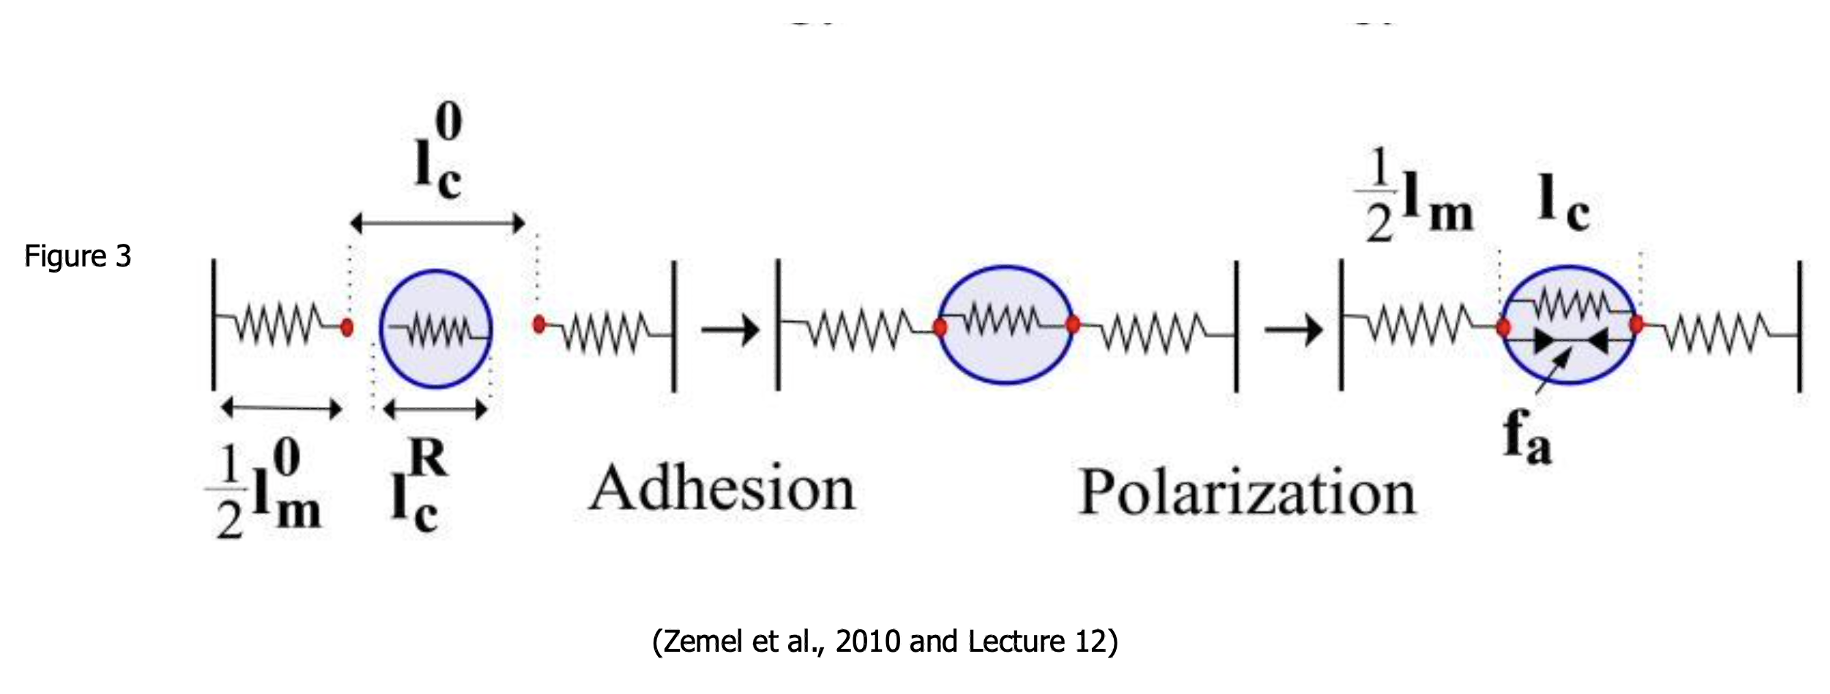
\includegraphics[width=1\textwidth]{springs}
  \caption{1D model: active cell spring (stiffness \(k_c\)) in series with 
  ECM spring (stiffness \(k_m\)).}
  \label{fig:1d-spring-model}
\end{figure}

\section*{Interpretation}

The formal form of anisotropic polarized actomyosin force is:
\[
  \frac{f^{a}}{f^{0}}
  = \alpha \,\frac{k_{m}}{\tilde{k}_{c} + k_{m}}
\]

\begin{itemize}
  \item $\displaystyle \alpha$: polarizability factor
  \item $\displaystyle \tilde{k}_{c} = (1 + \alpha)\,k_{c}$: effective stiffness of the cell
  \item $k_{m}$: matrix rigidity
\end{itemize}

\begin{itemize}
  \item For very soft matrices (\(k_{m}\ll \tilde{k}_{c}\)):
    \[
      \frac{f^{a}}{f^{0}}
      = \alpha \,\frac{k_{m}}{\tilde{k}_{c} + k_{m}}
      \;\longrightarrow\;0
      \quad\text{as }k_{m}\to 0.
    \]
    If \(k_{m}\ll \tilde{k}_{c}\), then \(\tilde{k}_{c}+k_{m}\approx \tilde{k}_{c}\) and
    \[
      \frac{f^{a}}{f^{0}}
      \approx \alpha \,\frac{k_{m}}{\tilde{k}_{c}}
       \approx   \alpha^{*}  \,k_{m}
      \;\longrightarrow\;0
      \quad\text{as }k_{m}\to 0.
    \]
  \item For very stiff matrices (\(k_{m}\gg \tilde{k}_{c}\)):
    \[
      \frac{f^{a}}{f^{0}}
      = \alpha \,\frac{k_{m}}{\tilde{k}_{c} + k_{m}}
      \approx \alpha \,\frac{k_{m}}{k_{m}} 
      \;\longrightarrow\;\alpha
    \] 
\end{itemize}

Thus, the active force grows with matrix stiffness and  
saturates at a maximum value proportional to~$\alpha$.

\begin{figure}[H]
  \centering
  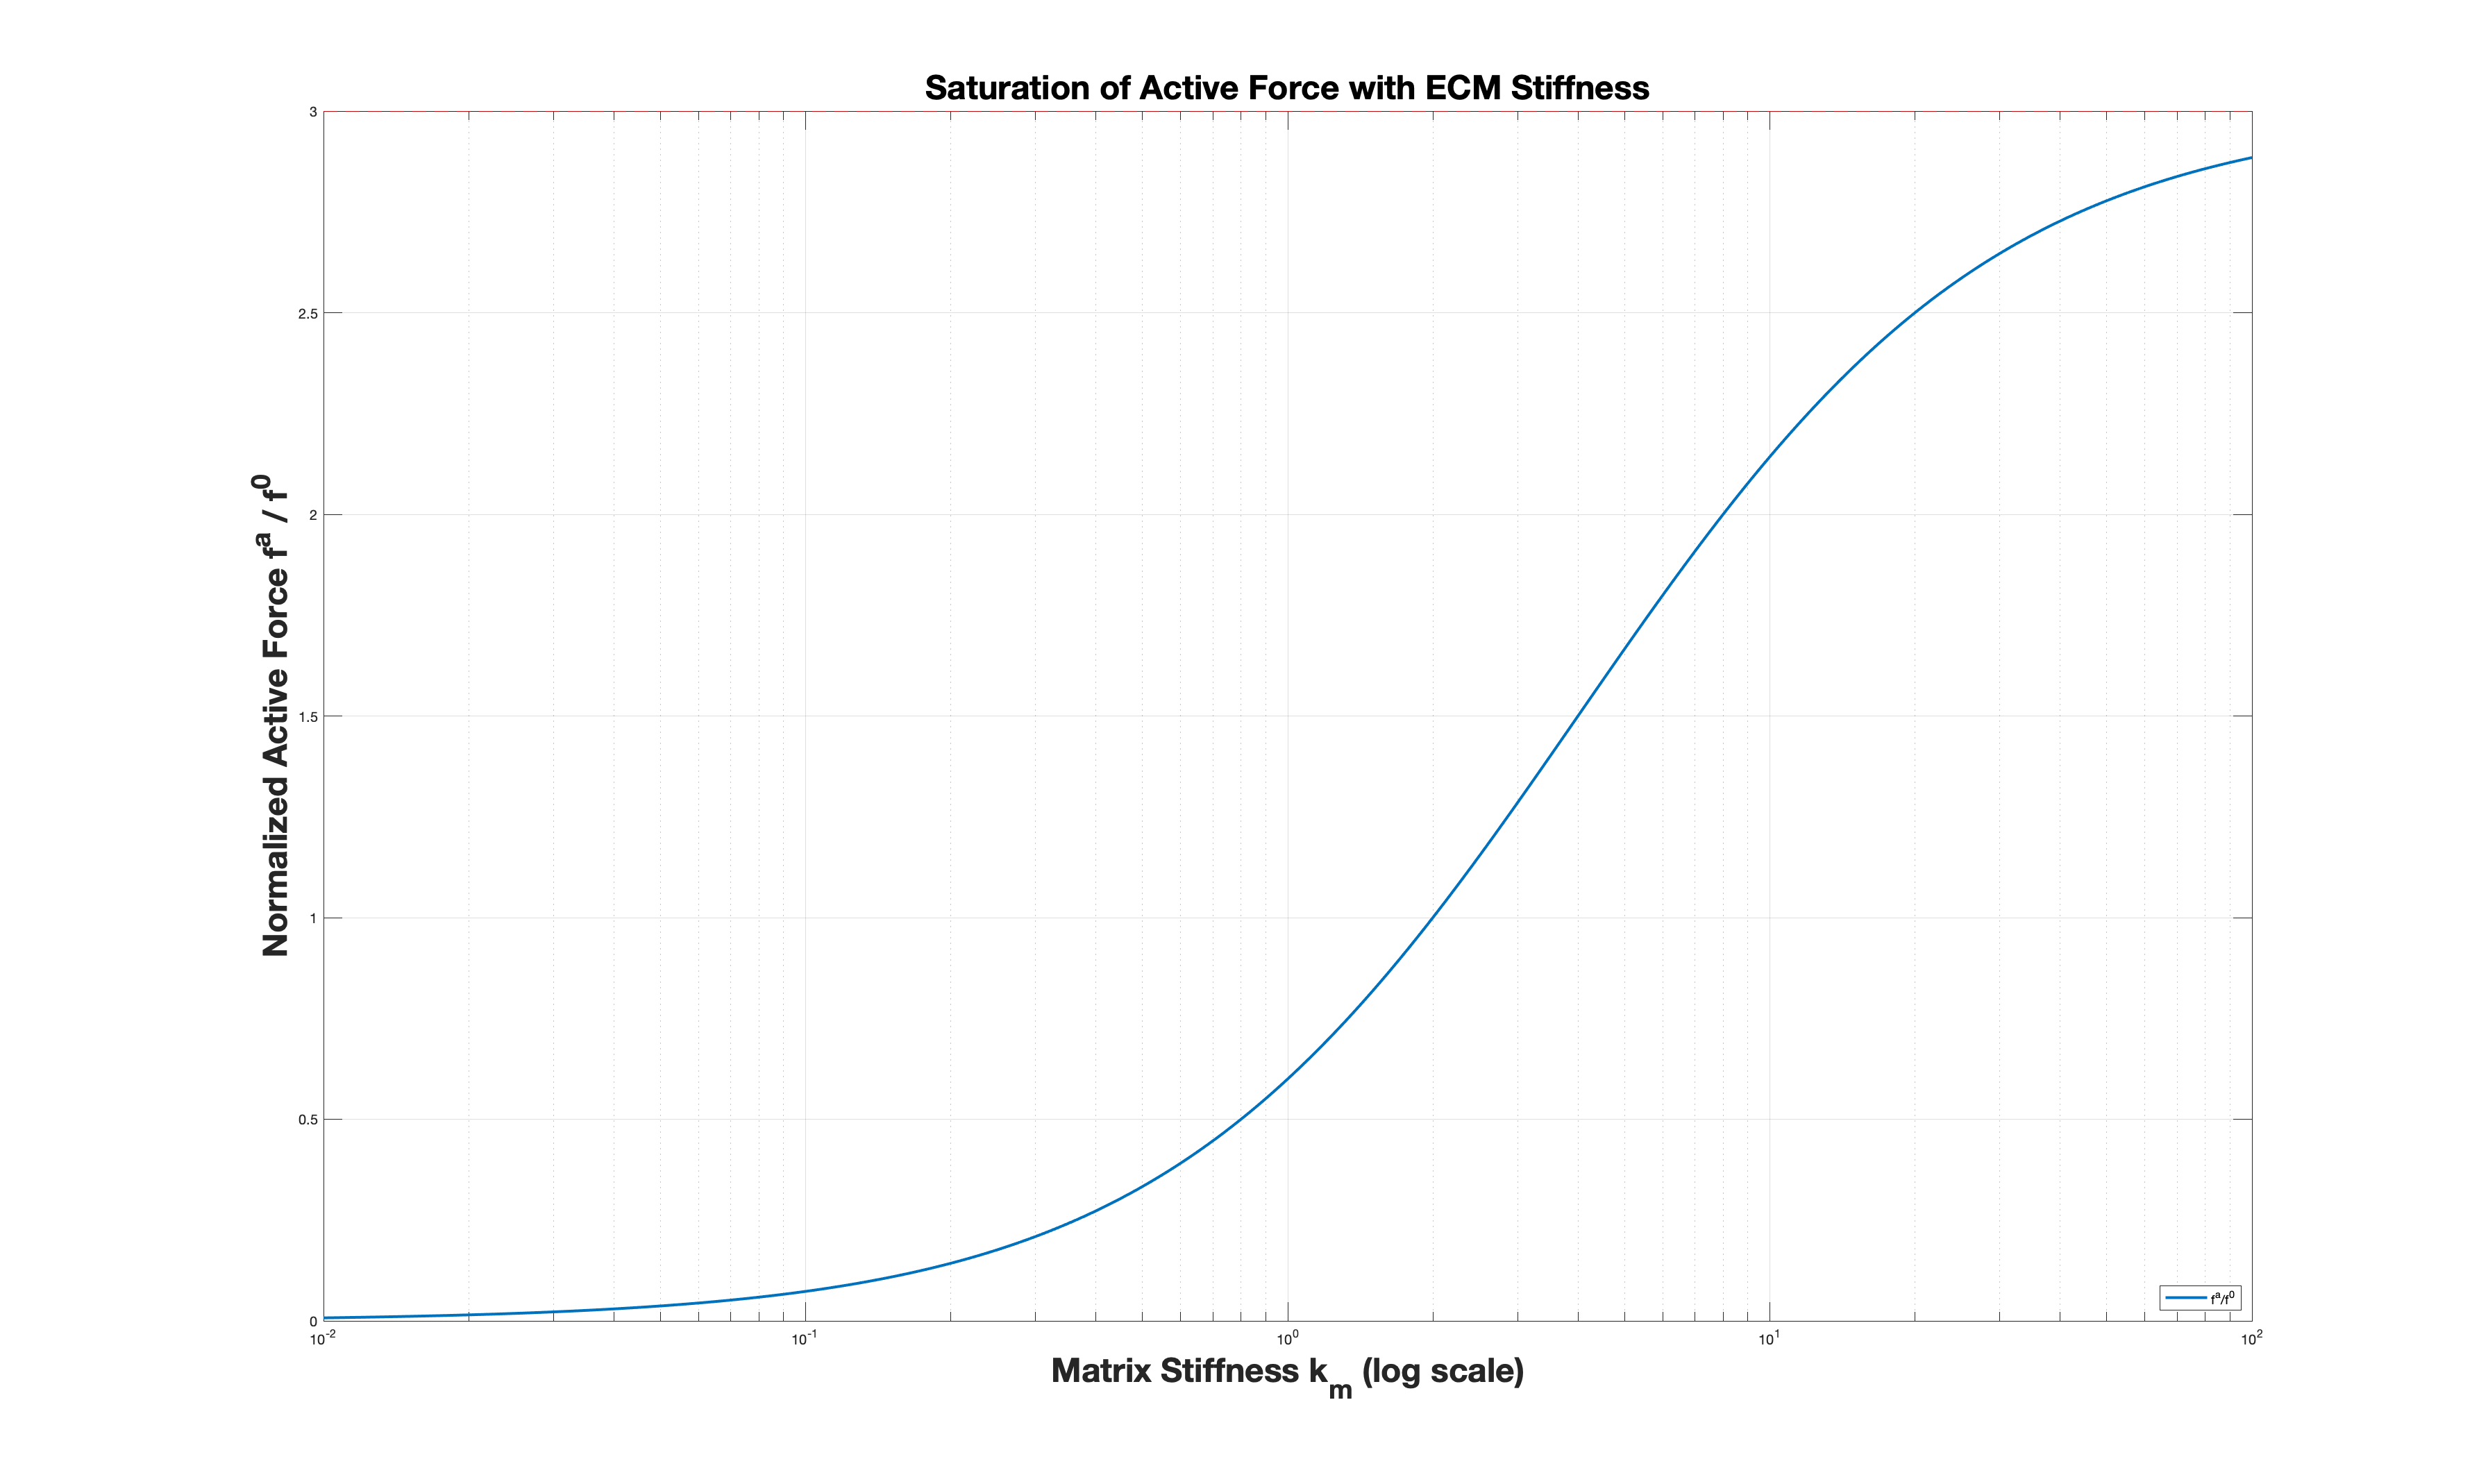
\includegraphics[width=0.8\textwidth]{plot}
  \caption{Active Force vs. Matrix stiffness.}
  \label{fig:activeForcet}
\end{figure}
     
\bibliographystyle{plain}
\bibliography{bibliography}

\end{document}
